% !TeX root = Proposal.tex
% !TeX encoding = UTF-8
% !TeX spellcheck = en_US

%=============================================================================
%
% This proposal will be written as an article
%
%=============================================================================
\documentclass[11pt,a4paper,titlepage]{article}

%opening
\title{Robust optimization and parameter estimation of queueing networks \\ PhD Research Proposal}
\author{Harold Ship \\ University of Haifa}

%=============================================================================
%
% This part of the preamble is the package importing and setup
%
%=============================================================================


% UTF file input
\usepackage[utf8]{inputenc}
\usepackage[T1]{fontenc}
\usepackage[english]{babel}

% math stuff
\usepackage[fleqn]{amsmath}
\usepackage{amsfonts} % for mathbb
\usepackage{mathtools} % loads amsmath plus other tools
\usepackage{fixmath} % fix greek letters
\usepackage{relsize} % for \mathlarger
\usepackage{bm} % for \bm which does bold in math mode
\usepackage[noend]{algpseudocode} % for algorithmics

% math theorems and theorem environments
\usepackage{amsthm}

% biblatex for references
\usepackage{csquotes} % ensures biblatex quotes things correctly
\usepackage[backend=biber,style=apa,autocite=inline]{biblatex}
\DeclareLanguageMapping{english}{english-apa}
\addbibresource{personal_bibliography.bib}

% puts hyperlinks in PDF. Must be loaded before cleveref
\usepackage{hyperref}
\hypersetup{hypertexnames=false}

% better cross-refs like Equations, etc
\usepackage{cleveref}

% Glossary, acronym
\usepackage[acronym,toc,nonumberlist]{glossaries}
\loadglsentries{glossary}
\makeglossaries

% drawings
\usepackage{tikz}
\usetikzlibrary{positioning}% To get more advances positioning options
\usetikzlibrary{arrows}% To get more arrow heads
\usetikzlibrary{shapes.geometric}% To get more shapes
\usetikzlibrary{fit}% To fit shapes inside shapes

\usepackage{paralist} % for compactlist
%=============================================================================
%
% My macros
%
%=============================================================================
\renewcommand*{\vec}[1]{\ensuremath{\bm{#1}}}%
\newcommand*{\mat}[1]{\ensuremath{\mathrm{#1}}}%
\newcommand*{\transpose}[1]{\ensuremath{#1^{\mathrm{T}}}}%
\newcommand*{\dd}{\ensuremath{\mathop{}\!\mathrm{d}}}%
\newcommand*{\dt}[1]{\ensuremath{#1^{\prime}}}%
\newcommand*{\R}{\ensuremath{\mathop{}\!\mathbb{R}}}%
\newcommand*{\RR}[1]{\ensuremath{\mathop{}\!\mathbb{R}^{#1}}}%
\newcommand*{\optimal}[1]{\ensuremath{#1^*}}%
\newcommand*{\uncertainset}[1]{\ensuremath{\mathcal{#1}}}%
\newcommand*{\defnterm}[1]{\textbf{#1}}%
% sclp math model macros
\newcommand*{\qnet}{\ensuremath{\mathcal{N}}}%
\newcommand*{\serv}{\ensuremath{i}}%
\newcommand*{\nserv}{\ensuremath{I}}%
\newcommand*{\class}{\ensuremath{j}}%
\newcommand*{\nclass}{\ensuremath{J}}%
\newcommand*{\queue}{\ensuremath{k}}%
\newcommand*{\nqueue}{\ensuremath{K}}%
\newcommand{\Tau}{\mathrm{T}}

% other macros
\newcommand\needc{{\color{purple}\textit{(citation needed)}}}
\newcommand\tbd{{\color{orange}\textit{TBD}}}

% math theorem environments (must be after cleveref)
\theoremstyle{definition}
\newtheorem{assumption}{Assumption}
\newcommand{\assumptionautorefname}{Assumption}
\newtheorem{example}{Example}
\newcommand{\exampleautorefname}{Example}
\theoremstyle{plain}
\newtheorem{claim}{Hypothesis}
\newcommand{\claimautorefname}{Hypothesis}



%=============================================================================
%
% This is where the document begins
%
%=============================================================================

\begin{document}


    \pagenumbering{roman}

    %=============================================================================
    % Make the title page and other boilerplate
    %=============================================================================
    \begin{titlepage}

        \begin{center}
            \linespread{1.5}
            {\large UNIVERSITY OF HAIFA} \medskip \\
            {\large DEPARTMENT OF STATISTICS} \vspace*{0.5cm} \\
            {\Large PhD RESEARCH PROPOSAL} \vspace*{2.0cm} \\
            \linespread{2}
            {\huge \textbf{Robust optimization and parameter estimation of queueing networks}} \vspace*{2.3cm}
        \end{center}

        \begin{minipage}[t]{0.5\textwidth}
            \begin{flushleft}
                {\large \textit{Author}:\vspace*{0.5cm} \\ Harold Ship \\
                    324698703
                }
            \end{flushleft}
        \end{minipage}%
        %
        \begin{minipage}[t]{0.5\textwidth}
            \begin{flushright}
                {\large \textit{Supervisors}:\vspace*{0.5cm} \\Dr. Itai Dattner\vspace*{0.1cm}\\Dr. Evgeny Shindin\\
                }
                \vspace*{0.5cm}
            \end{flushright}
        \end{minipage}%

        \begin{center}
            \begin{minipage}[b]{0.5\textwidth}
                \vfill
                \begin{center}
                    {\large 10 October 2021}
                \end{center}
            \end{minipage}%
        \end{center}

        \thispagestyle{empty}

    \end{titlepage}



    %=============================================================================
    % Make the other boilerplate
    %=============================================================================

    \tableofcontents \clearpage
    \iffalse % remove to enable list of figures
    \listoffigures \clearpage
    \fi
    \iffalse % remove to enable list of tables
    \listoftables \clearpage
    \fi
    \printglossaries \clearpage


    \pagenumbering{arabic}
    \setcounter{page}{1}

    % these styles are for tikz drawings in this section
    \tikzstyle{server}=[%
    rectangle,
    minimum height=3cm,
    %rounded corners=4pt,
    text height=0.75cm,
    text depth=.5cm,
    text width=1cm,
    inner xsep=1em,
    inner ysep=1.5em,
    text centered,
    draw=black!50
    ]
    \tikzstyle{server-label}=[%
    fill=white,
    font=\scriptsize
    ]
    \tikzstyle{vserver}=[%
    rectangle,
    rounded corners,
    minimum height=3cm,
    %rounded corners=4pt,
    text height=0.75cm,
    text depth=.5cm,
    text width=1cm,
    inner xsep=1em,
    inner ysep=1em,
    text centered,
    draw=black!50,
    fill=black,
    fill opacity=0.1
    ]
    \tikzstyle{buffer}=[%
    rectangle,
    minimum height=1cm,
    %rounded corners=4pt,
    text height=0.75cm,
    text depth=.5cm,
    text width=1cm,
    text centered,
    font=\scriptsize,
    inner sep=0pt,
    draw=red!20,
    fill=red!20
    ]
    \tikzstyle{buffer-label}=[%
    draw=red!50,
    fill=white,
    font=\tiny
    ]
    \tikzstyle{input}=[%
    rectangle,
    minimum height=1cm,
    %rounded corners=4pt,
    text height=0.75cm,
    text depth=.5cm,
    text width=1.5cm,
    text centered,
    inner sep=0pt,
    draw=white!0,
    fill=white!0
    ]
    \tikzstyle{output}=[%
    rectangle,
    minimum height=1cm,
    %rounded corners=4pt,
    text height=0.75cm,
    text depth=.5cm,
    text width=1cm,
    text centered,
    inner sep=0pt,
    draw=white!0,
    fill=white!0
    ]
    \tikzstyle{task}=[%
    rectangle,
    minimum height=1cm,
    %rounded corners=4pt,
    text height=0.75cm,
    text depth=.5cm,
    text width=1cm,
    text centered,
    inner sep=0pt,
    draw=black!50,
    fill=orange!20
    ]
    \tikzstyle{taskflow}=[%
    semithick,
    blue,
    below,
    ->,
    >=stealth
    ]

    %=============================================================================
    % Introduction
    %=============================================================================
    \section{Introduction}
    \label{sec:introduction}


    Many problems in queueing theory consist of multiple classes of jobs
    that are processed by a network of servers.
    We often model such problems as \Glspl{mcqn}.
    Optimizing \glspl{mcqn} directly is intractable,
    but in many cases a near-optimal solution can be found by approximating the jobs as fluids.
    One such method produces a \gls{sclp} problem,
    which we can solve using the SCLP-Simplex method.


    While the SCLP-Simplex method has been demonstrated for solving the general \gls{mcqn} problem,
    there are some variations where the algorithm may require some improvement.
    In particular,
    the details of the job arrival process and the job processing process are often not known exactly.
    They may also vary over time.

    This document proposes research for a PhD in Statistics at University of Haifa in the area of \gls{mcqn} with uncertain data.
    We plan to cover four general problems,
    described in detail in \Cref{sec:topics}.
    We plan to extend the \gls{sclp}-Simplex algorithm to handle uncertainty budgets (\Cref{subsec:topics:robust-sclp-extension}),
    to improve on \autocite{bertsimas2014robust} robust model for \gls{mcqn} optimal control problems where the natural control variables are server effort (\Cref{subsec:topics:enhanced-robust-sclp}),
    develop an iterative method for simultaneously optimizing a \gls{mcqn} and learning its parameters (\Cref{subsec:topics:iterative}),
    and extend \gls{sclp}-Simplex for piece-wise constant arrival rates and processing times,
    including estimatation of these parameters (\Cref{subsec:topics:sclp-piecewise}).
    In \cref{sec:results} we present some preliminary results.


    \example{
        \label{ex:one-computer-concrete}
        Suppose we have single computer that will be used to run jobs over the next $T=10$ hours (\Cref{fig:one-computer-concrete}).
        It takes $\tau=1$ minute to complete each job,
        so the computer can service $\mu=60$ jobs per hour.
        Meanwhile, additional jobs arrive at a constant rate of $\lambda=40$ per hour.
        The computer has a queue for waiting jobs which has $x(t)$
        jobs in it at time $t$,
        and starts with $x(0)=100$ jobs in it.

        If we let the computer work at $100\%$ of its capability,
        then after five hours ($100 + 40 t = 60 t \implies t = 5$) the queue will be empty.
        We can then let the computer work at $66.67\%$ for the next five hours,
        so that it processes jobs at the rate they arrive,
        or $40$ jobs per hour.
        In this way it will keep the queue empty.

        \begin{figure}
            \centering
            \resizebox{\textwidth}{!}{
                \begin{tikzpicture}[node distance=2.5cm]
                    % Server nodes
                    \node[buffer] (B) at (0,0) {$x(t)$};
                    \node[buffer-label] at (B.north) {$B$};
                    \node[input] (I) [left of=B] {};
                    \node[output] (O) [right of=B] {};
                    \node[server,fit=(B)] (S) {};
                    \node[fill=white] at (S.north) {$S$};
                    % Network flow paths
                    \path[taskflow] (I) edge node {$40$} (B);
                    \path[taskflow] (B) edge node {$60$} (O);
                \end{tikzpicture}
            }% resizebox
            \caption[Single computer with constant job rate.]{
                \label{fig:one-computer-concrete}
                A single computer server $S$ with constant job arrival rate of $40$ jobs per hour.
                The computer contains a job queue $B$ containing $x(t)$ jobs at time $t$.
                It services the jobs at rate $60$ jobs per hour,
                after which they exit the system.
            }
        \end{figure}
    }

    \example{
        \label{ex:one-computer-two-classes-concrete}
        Our next example builds on \Cref{ex:one-computer-concrete}
        by adding a second job class serviced by the same computer.
        For this second class,
        jobs arrive at $20$ per hour to a second job queue,
        and it takes $2.4$ minutes to complete each job so that they
        and are processed at $25$ jobs per hour.
        The job queue for the second job class starts with $100$ jobs in it.
        \Cref{fig:one-computer-two-classes-concrete} illustrates this setup.

        With two classes,
        it is possible that the holding cost of waiting in the queue is different for each class.
        But for now,
        we assign a cost per unit time of $1$ to each buffer,
        and try to minimize the objective function

        \begin{equation}
            \label{eq:one-computer-two-classes-concrete-objective}
            z = \int\limits_0^T \left( x_1(t) + x_2(t) \right) \dd{t}.
        \end{equation}

        The length of the queues $B_1, B_2$ depends on three things:
        jobs arriving at the queue,
        jobs being processed by the server,
        and the initial quantity at time $t=0$.
        Since we now require the computer to work on two job classes,
        we introduce the control variables $\eta_1(t), \eta_2(t)$
        which allow us to specify how much effort to apply to each job class
        at time $t$.
        The server $S_1$ has a maximum rate it can operate,
        which we normalize to $1$.
        This gives us the following constraints,
        which must hold for all $t \in [0,T]$:
        \Cref{eq:one-computer-two-classes-concrete-server-constraints} on the server and
        \Cref{eq:one-computer-two-classes-concrete-balancing-constraints} constrains the queue lengths $x_1(t), x_2(t)$ at time $t$.

        \begin{align}
            \label{eq:one-computer-two-classes-concrete-server-constraints}
            0 \leq \eta_1(t) + \eta_2(t) & \leq 1
        \end{align}

        \begin{align}
            \label{eq:one-computer-two-classes-concrete-balancing-constraints}
            \begin{split}
                x_1(t) & = 100 - \int\limits_0^t 60 \eta_1(s) \dd{s} + 40 t \geq 0 \\
                x_2(t) & = 100 - \int\limits_0^t 25 \eta_2(s) \dd{s} + 20 t \geq 0
            \end{split}
        \end{align}

        If we define the matrices
        $
        G =
        \begin{bmatrix}
            60 & 0 \\
            0 & 25
        \end{bmatrix}
        $
        and
        $
        H =
        \begin{bmatrix}
            1 & 1
        \end{bmatrix}
        $,
        and the vectors
        $
        c = (1,1)^\top
        $,
        $
        \alpha = (100,100)^\top
        $,
        $
        a = (40,20)^\top
        $,
        $
        b = (1)^\top
        $,
        $
        \eta(t) = (\eta_1(t), \eta_2(t))^\top
        $,
        and
        $
        x(t) = (x_1(t), x_2(t))^\top
        $

        we derive the following \gls{sclp} minimization problem:

        \begin{align}
            \begin{split}
                \min\limits_{u}
                &~ = \int_0^T c^\top \eta(t) \mathrm{d}t \\
                \text{s.t.}
                &~ \int_0^t G \eta(s) \mathrm{d}s \leq \alpha + a t \\
                &~ H \eta(t) \leq b \\
                &~ \eta(t) \geq 0
            \end{split}
        \end{align}

        \begin{figure}
            \centering
            \resizebox{\textwidth}{!}{
                \begin{tikzpicture}[node distance=1cm]
                    % buffer nodes
                    \node[buffer] (B1) at (0,0) {$x_1(t)$};
                    \node[buffer-label] at (B1.north) {$B_1$};
                    \node[buffer] (B2) [below=of B1] {$x_2(t)$};
                    \node[buffer-label] at (B2.north) {$B_2$};
                    % input and output nodes
                    \node[input] (I1) [left=2.5cm of B1] {};
                    \node[input] (I2) [left=2.5cm of B2] {};
                    \node[output] (O1) [right=2.5cm of B1] {};
                    \node[output] (O2) [right=2.5cm of B2] {};
                    % server nodes
                    \node[server,fit=(B1)(B2)] (S1) {};
                    \node[server-label] at (S1.north) {$S_1$};
                    % Network flow paths
                    \path[taskflow] (I1) edge node {$40$} (B1);
                    \path[taskflow] (I2) edge node {$20$} (B2);
                    \path[taskflow] (B1) edge node {$60$} (O1);
                    \path[taskflow] (B2) edge node {$25$} (O2);
                \end{tikzpicture}
            }% resizebox
            \caption[One computer with two job classes.]{
                \label{fig:one-computer-two-classes-concrete}
                One computer server with two job classes.
                The jobs arrive at the constant rates of
                $40$ and $20$ jobs per hour respectively for each class.
                Jobs from each class wait in corresponding queues $B_1, B_2$
                containing $x_1(t), x_2(t)$ jobs at time $t$, respectively.
                The computer services the jobs at rates
                $60$ and $25$ jobs per hour for the two classes.
            }
        \end{figure}
    }

    % =============================================================================
    % Theory
    % =============================================================================
    \section{Theory}
    \label{sec:theory}

    % =============================================================================
    % Multi-class Queueing Networks
    % =============================================================================
    \subsection{Multi-class Queueing Networks}
    \label{subsec:theory:mcqn}

    In queueing theory,
    jobs that arrive at queues,
    and are then processed by servers.
    We model the arrival of jobs at queues as well as the processing
    as stochastic processes.
    A \Gls{mcqn} is a system in there are several classes of jobs.
    Each class has an arrival stochastic process,
    a processing stochastic process,
    a dedicated server,
    a holding cost per unit time,
    a processing cost per unit time,
    and a set of child jobs that are generated when the job has been completed.
    Servers typically process more than one job class,
    and so have several associated queues.
    A common issue with such a system is to decide,
    at a given time $t$,
    which job class to process on each server.
    Alternatively,
    we can decide what fraction of its processing capacity each server will dedicate to
    each job class.


    \Glspl{mcqn} typically consist of large numbers of job classes,
    queues,
    and servers.
    Furthermore,
    there may be child-jobs that need to run on different servers,
    and so the decisions taken on separate servers are dependent on one another.
    Because of this,
    and the stochastic nature of the arrivals and processing times,
    optimizing the cost of a \gls{mcqn} is an intractable problem.
    A common technique for overcoming this problem is
    to approximate the stochastic arrival and server-processing processes
    as constant rate fluid flows \autocite{weiss1999scheduling}.
    We can then model the \gls{mcqn} as a \Gls{sclp},
    and then solve it with one of several algorithms.

    % =============================================================================
    % The Workload Placement Problem
    % =============================================================================
    \subsection{The Workload Placement Problem}
    \label{subsec:theory:workload-placement}

    For example,
    the workload placement problem is real-world problem that we can model using \gls{mcqn},
    and solve using \gls{sclp}.
    New applications based on the \gls{iot} are often too large to run on a single machine.
    They must be divided into separate jobs that run on multiple computing devices that live both in a Cloud system and close to the \gls{iot} devices -- on the Edge.

    The efficient assignment of jobs to computing devices in cloud and edge networks is a difficult computational problem in optimization and optimal control,
    known as the Workload Placement Problem.
    Today,
    the workload placement problem is usually solved one job at a time \autocite{10.1145/3391196,youssef_2020}:
    a scheduler process takes one or more jobs from an input stream,
    examines the state of all the servers,
    decides to which server queues to place those jobs.
    However,
    this may not make optimal use of the servers' resources.

    % =============================================================================
    % State of the Art
    % =============================================================================
    \subsection{State of the Art}
    \label{subsec:theory:state_of_the_art}

    A review of \autocite{bertsimas2014robust}.

    A \gls{mcqn} is a system for processing jobs,
    which are divided into classes.
    Each job in a class has the same arrival rate,
    processing time,
    a cost per unit time for holding it in its queue and for processing it,
    and a defined path through the network.
    In order to find the optimal job to process at each server,
    one must know the current state of all the queues on that server,
    and also the states of other servers that feed into and out of the server.
    These problems quickly become large and difficult to solve.

    %Most often,
    %the processing times and arrival rates are known with some degree of uncertainty.
    %This adds further complexity to the problem.
    %\autocite{bertsimas2014robust} lists several attempts to solve \gls{mcqn} with uncertain parameters.
    %The problem can be formulated as a ``stochastic dynamic programming'' problem.
    %However,
    %this method is intractable for large problems.
    %
    %
    %\begin{itemize}
    %    \item stochastic dynamic programming,
    %    but problems quickly become intractable,
    %    \item Brownian approximation models and
    %    \item fluid approximations
    %\end{itemize}

    Real-life optimization problems often have uncertain parameters,
    that is, they are not known exactly.
    For fluid processing networks these are the job arrival and service rates.
    These rates can also vary over time.
    One way to deal with uncertain parameters is to apply a Robust Optimization methodology.
    Robust optimization considers that part of the problem parameters can deviate from their nominal values taking the values in the some set,
    called the uncertainty set.
    Based on the original (nominal) problem and on the uncertainty set Robust Optimization allows
    \Autocite{bertsimas2014robust} to develop such a model for
    %\gls{mcqn} with the fluid approximation.
    fluid processing networks.
    They consider budgeted uncertainty sets for the arrival and service rates.
    The realized arrival rates and service times for class $i$ are
    defined as $\lambda_i(t), \tau_i(t)$ respectively.
    For $t in [0,T]$,
    $\tau_i(t) \in [\bar{\tau}_i, \tilde{\tau}_i]$ and
    $\lambda_i(t) \in [\bar{\lambda}_i, \tilde{\lambda}_i]$.
    Call $\bar{\tau}_i$ and $\bar{\lambda}_i$ the nominal arrival rate and service time.
    Call $\tilde{\tau}_i$ and $\tilde{\lambda}_i$ the deviation arrival rate and service time,
    and $z_i(t)$, $\zeta_i(t)$ the relative deviations.
    $z_i(t)$ is defined as

    \begin{equation}
        z_i(t) =
        \begin{cases}
            \frac{\tau_i(t) - \bar{\tau}_i}{\tilde{\tau}_i} & \tilde{\tau}_i > 0 \\
            0 & \text{otherwise.}
        \end{cases}
    \end{equation}
    $\zeta_i(t)$ is defined analogously for $\lambda$.
    If we take the deviations from all of the service times,
    the total service time deviation per server may be bounded by a ``budget''
    parameter $\Gamma_j$ for server $j$,
    and then we define an uncertainty set as follows:
    \begin{equation}
        \begin{split}
            &\tau_{i}(t)=\bar{\tau}_{i}+z_{i}(t) \tilde{\tau}_{i}, \quad \forall i, t \\
            &\sum_{i: s(i)=j} z_{i}(t) \leq \Gamma_{j}, \quad \forall j, t \\
            &0 \leq z_{i}(t) \leq 1, \quad \forall i, t
        \end{split}
    \end{equation}


    As a result, they derive a Robust Counterpart that is also an SCLP problem,
    and is formulated in \Cref{eq:mcqn-robust-counterpart}.
    This problem requires additional decision variables $\alpha_i(t), \beta_i(t)$
    for $i=1,\ldots,I$ servers.
    These variables have no physical meaning,
    but are necessary for the robust formulation.

    \begin{align}
        \begin{split}
            \label{eq:mcqn-robust-counterpart}
            \min & \int_{0}^{T} \mathbf{c}^{\prime} \mathbf{x}(t) d t \\
            \text { s.t. } & \int_{0}^{t} \mathbf{A} \mathbf{u}(s) d s+\mathbf{x}(t)=\mathbf{x}(0)+\overline{\boldsymbol{\lambda}} t, \quad \forall t \\
            & \Gamma_{j} \beta_{j}(t)+\sum_{i: s(i)=j}\left(\bar{\tau}_{i} u_{i}(t)+\alpha_{i}(t)\right) \leq 1, \quad \forall j, t, \\
            & \alpha_{i}(t)+\beta_{j}(t)-u_{i}(t) \tilde{\tau}_{i} \geq 0, \forall j, i \text { with } s(i)=j, \quad \forall t \\
            & \mathbf{u}(t), \mathbf{x}(t), \boldsymbol{\alpha}(t), \boldsymbol{\beta}(t) \geq \mathbf{0}, \quad \forall t
        \end{split}
    \end{align}



    % =============================================================================
    % Proposed Research Topics
    % =============================================================================
    \section{Proposed Research Topics}
    \label{sec:topics}

    In this section,
    we discuss proposed topics for research.
    The context is a \gls{mcqn}.
    We assume that the arrival rates $\lambda$
    and the processing rates $\mu$ of the job classes are unknown,
    although we may have initial estimates for these.
    We will observe a system over a specified time period which we call $t \in [0,T]$.
    We take samples at predetermined,
    fixed time intervals $m=1,\ldots,M$,
    of $\lambda(t_n)$,
    the observed number of arrivals by time $t_n$,
    and $\mu(t_n)$,
    the observed number of processed jobs by $t_n$.
    For example,
    when $N=1$,
    we can estimate the mean arrival and processing rates.

    \subsection{Extension of the SCLP-Simplex Algorithm to Budgeted Robust Optimization of MCQN}
    \label{subsec:topics:robust-sclp-extension}

    In the case where the uncertainty set and nominal value of the parameters is known,
    but there is still some uncertainty about how they will be realized,
    we hope to show that

    The solution method for the SCLP problem (\ref{eq:mcqn-robust-counterpart}) suggested in \autocite{bertsimas2014robust}
    is an algorithm of \autocite{luo1998new}
    that is based on time discretization and quadratic programming.
    However,
    \autocite{shindin2021application} show that solution methods based on time discretization are not good for the following reasons:
    \begin{compactitem}
        \item
        There is a trade-off between optimality of the solution and computation time,
        controlled by the fineness of the discretization,
        which may not have a satisfactory choice.
        \item
        It is difficult perform sensitivity analysis or adapt the solution to changes in the parameters of the optimization problem.
    \end{compactitem}
    Alternatively, one can use the SCLP-simplex \autocite{weiss2008simplex}
    or the Revised SCLP-simplex \autocite{shindin2021application}
    algorithm to solve this kind of problem.
    However, in the  robust  counterpart of the uncertain SCLP problem with budgeted uncertainty set (\ref{eq:mcqn-robust-counterpart}) third set of constraints has zero-valued right-hand-side.
    This means that the resulting SCLP problem is degenerate and neither SCLP-simplex,
    nor revised SCLP-simplex are designed to deal with degenerate SCLP problems.
    In LP,
    the standard way to handle degeneracy is to perturb the right-hand-side
    of the constraints with small values.
    However in SCLP, this may produce a large number of short intervals.
    This can slow down the algorithm creating a lot of spurious basic variables that vanishing after the short period.
    To avoid this issue,
    we propose to modify the SCLP-simplex algorithm in a way that will allow handling degeneracy without a need for perturbing the right hand side.


    \subsection{Enhanced, Relaxed Robust SCLP for certain cases of MCQN}
    \label{subsec:topics:enhanced-robust-sclp}


    Bertsimas model (\ref{eq:mcqn-robust-counterpart})
    produces a so-called  ``sequencing policy'' that decides on the priority of each job as it arrives.
    In some cases,
    we cannot implement such a policy due to the nature of the problem.
    For example,
    in the Workload Placement Problem,
    one usually controls how much of various resources to allocate to
    each job.
    Thus,
    instead of the ``sequencing policy'' one could implement a ``server-effort policy'' that controls the server effort per job class.
    In the Workload Placement Example,
    we could control the percent of CPU to dedicate to each class.

    In the deterministic case the optimal sequencing policy and optimal server-effort policy are interchangeable,
    i.e. one could be obtained from another by algebraic manipulation.
    For the robust optimization problem this is not true,
    because service rates are uncertain and then the resulting sequencing policy will depend on realization of these parameters.
    To avoid this issue we propose to use the server-effort problem formulation,
    where the control variables are formulated directly as a percent of the server effort,
    and derive robust counterparts for this problem formulation for a variety of uncertainty set shapes,
    including  box, budgeted and polyhedral uncertainty sets.
    We believe that the corresponding robust counterparts will be \gls{sclp} problems as well.
    We believe that the value of the holding cost objective for this formulation will always be as low as or lower than the sequencing-policy formulation.
    We plan to demonstrate this by comparing the feasible regions of the corresponding robust counterparts,
    and showing that the proposed model's region contains the feasible region of Bertsimas' model.

    A Robust Solution is feasible for any value of parameters realized from the uncertainty set.
    This includes the worst case values,
    meaning the parameters for which the solution is furthest from optimal.
    The uncertainty sets do not require any knowledge or assumptions about the distributions of the parameters.
    In many situations,
    it may be possible to make use of other information about the parameters,
    to obtain a more optimal solution.
    We plan to use the expected values of the arrival and service rates in order to build the relaxed \gls{sclp} problem mentioned above and investigate the quality of the resulting policy under different distributions of these rates.


    The robust policy enforces constraints on the buffers,
    such that they must be non-negative for all possible realizations of the parameters.
    However,
    in some examples such as the Workload Placement Problem,
    the server can handle empty buffers by simply not working on this buffer.
    This means that we can relax the constraints that require the buffers to be non-negative under all possible realizations of the parameters.
    We believe that such a relaxation will achieve an as-good or better objective value,
    because a relaxation of the constraints increases the feasible region.
    We hope to show that under certain conditions,
    % {\color{red} such as that the primary source of uncertainty is deviation from the nominal over time,}
    including when the nominal values of uncertain parameters considered to be equal to their expected values,
    this robust objective approaches the nominal or deterministic objective.
    We plan to demonstrate this theoretically and experimentally.
    Experimentally,
    we can use Monte Carlo methods on a set of Robust Problems.
    Theoretically,
    we plan to find how the distribution of the parameters propagates to the distributions of the realized values of the objective function and to the corresponding solution.
    Alternatively,
    we can use a stochastic programming approach to show that the objective of the relaxed problem is better than that of the original problem.
    We have some preliminary experimental results in \Cref{sec:results}.

    \subsection{Iterative Algorithm for Solving MCQN with Uncertain Parameters}
    \label{subsec:topics:iterative}


    In the previous section,
    we discussed a server-effort policy that we believe will consistently produce better results than a sequence policy for certain problems in the presence of uncertain parameters,
    in particular when the uncertainty set is well known.
    In this section,
    we consider a more general case,
    when we have very little information about these parameters at all,
    or when the uncertainty set is too big.
    It may in fact be too big for a robust solution to exist.
    Another case is where we have an estimate for the expected values of some of these parameters,
    but the confidence interval is large.
    Consequently,
    in addition to optimizing the system,
    we would like to improve our knowledge about the parameters and uncertainty sets.
    Better knowledge of the parameters will allow us to create a more accurate mathematical model of the problem,
    and consequently obtain a better control policy.

    We propose to develop an iterative algorithm that at each step
    alternates between producing a new solution from the uncertain set of parameters,
    and learning about those parameters in order to improve the solutions of subsequent steps.
    We begin with
    an initial control policy,
    such as the robust control policy if one exists,
    based on the the uncertainty set of the parameters.
    This policy would be optimal according to the initial knowledge about the uncertain parameters,
    and moreover,
    it would allow for the system to be deployed and run.
    Before running it,
    however,
    we perform a sensitivity analysis on the uncertain parameters in order to discover which parameters have the greatest effect the objective.
    We plan to develop statistical methods to perform the estimation of the uncertainty set and expected values of those parameters.
    These methods will result in a control policy that enables us to estimate the parameters in some confidence intervals.
    This policy has a price which can be calculated from the objective function of the optimization problem.
    Next,
    we create a combined policy by taking the weighted sum of estimator policy and the robust policy,
    using weights which we set.
    There is an inherent trade-off between the estimator policy and the robust policy.
    On the one hand,
    the estimator policy will often be closer to optimal,
    given that the robust solution covers the worst case.
    On the other hand,
    the estimator policy will enable better parameter estimation.
    We run the system over a period $[0,T]$,
    and measure the number of job arrivals and completions for each class.
    We use these to estimate the expectations and/or uncertainty sets for the arrival rates and processing times $\hat{\lambda}_j, \hat{\tau}_j$ for each class $j$,
    and then generate a new robust policy based on the estimated parameters.


    The method we use to compute the estimator policy will be investigated as part of this research topic.
    Since the SCLP-Simplex algorithm is centered on an \gls{ode} containing our parameters,
    we plan to base our parameter estimation approach on the direct integral method \autocite{dattner2015optimal,dattner2015model,yaari2018simode}.
    We believe this method will allow us to estimate the parameters in our partially observed system,
    because although it is not hard to estimate the arrival rates $\lambda$,
    the processing times or rates for job classes may be difficult to measure directly.
    Instead,
    we usually must measure the length of each queue $x(t)$.

    We can repeat this process until we are satisfied with the parameter estimates.



    \subsection{Extend proposed techniques for the problems with Piecewise Constant arrival and service rates}
    \label{subsec:topics:sclp-piecewise}
    \subsubsection{Extension of SCLP-simplex algorithm}
    The SCLP-Simplex algorithm can solve MCQN problems,
    for which the arrival and processing stochastic processes are homogeneous
    with corresponding constant rates in the fluid approximations.
    In order to apply the algorithm to a wider range of stochastic processes,
    constant values for these quantities may not make sense.
    One possible extension would be to use piece-wise constant values.
    However,
    it is well known that strong duality between SCLP and its symmetric dual does not hold when the arrival and service rates are piece-wise constant.
    Using a non-symmetric dual does not substantially change the theory \autocite{pullan1993algorithm,shapiro2001duality},
    however impulses at breakpoints may appear in the dual problem at places where problem parameters have breakpoints.

    To resolve this issue we plan to adapt the theory and the simplex-type algorithm that developed for M-CLP problems \autocite{shindin2014symmetric,shindin2015structure,shindin2020simplex}, which may posses impulses at the beginning and at the end of time interval.

    \subsubsection{Extension of parameter estimation methods}
    We expect that estimating these piece-wise constant parameters when they are known with some degree of uncertainty will be challenging.
    We plan to investigate changepoint detection algorithms and other time series analysis techniques in combination with parameter estimation for \glspl{ode} based on the direct integral method \autocite{dattner2015optimal,dattner2015model,yaari2018simode}, in order to estimate the locations and values of the changes of the ``pieces''.

    % =============================================================================
    % Preliminary Results
    % =============================================================================
    \section{Preliminary Results}
    \label{sec:results}

    \newcommand{\modelone}{Model 1}
    \newcommand{\modeltwo}{Model 2}

    This section describes the preliminary experimental work towards the research topic \Cref{subsec:topics:robust-sclp-extension},
    which we performed using the setup of \Cref{ex:one-computer-two-classes-concrete}.
    We begin by comparing our proposed model,
    which we call \modelone,
    to Bertsimas' model,
    which we call \modeltwo.
    First, we show that the two deterministic versions of the model are equivalent.
    Then,
    we look at what happens when we introduce some uncertainty to the processing time parameter $\tau$.
    Then we show how we can make adjustments to \modelone that improve the objective significantly.


    First we solve the deterministic version of our \modelone.
    This model uses the fraction of effort $\eta$ on the server as the decision variables.

    \begin{align}
        \label{eq:model-1}
        \begin{split}
            \min\limits_{\eta_1, \eta_2}
            &~ \int_0^T \left( x_1(t) + x_2(t) \right) \dd t \\
            \text{s.t.}
            &~ 0 \leq \eta_1(t) + \eta_2(t) \leq 1 \\
            &~ x_1(t) = 100 - \int_0^t 60 \eta_1(s) \dd s + 40t \geq 0 \\
            &~ x_2(t) = 100 - \int_0^t 25 \eta_2(s) \dd s + 20t \geq 0
        \end{split}
    \end{align}

    The optimal solution,
    obtained using the SCLP-Python solver \autocite{Shindin_SCLPPython_2021},
    has the server applying $100\%$ effort on class 1 jobs for the first $5$ hours,
    then $66.67\%$ on class 1 and 33.33\% on class 2 for the last 5 seconds.
    The value of the objective is $2145.83$.

    We define a second model,
    based on the model of \autocite{bertsimas2014robust},
    which we call \modeltwo.
    Define  decision variables $u_1(t), u_2(t)$ as the task flow rates
    in tasks per unit time.
    The server effort is still constrained at $100\%$,
    and so we translate the constraints according to the formulas:
    \begin{align}
        \label{eq:model-2-translation}
        \begin{split}
            u_1(t) & = 60 \eta_1(t) ~ \text{and} \\
            u_2(t) & = 25 \eta_2(t).
        \end{split}
    \end{align}

    The following model is the result:

    \begin{align}
        \label{eq:model-2}
        \begin{split}
            \min\limits_{u_1, u_2}
            &~ \int_0^T \left( x_1(t) + x_2(t) \right) \dd t \\
            \text{s.t.}
            &~ 0 \leq \frac{u_1(t)}{60} + \frac{u_2(t)}{25} \leq 1 \\
            &~ x_1(t) = 100 - \int_0^t u_1(s) \dd s + 40t \geq 0 \\
            &~ x_2(t) = 100 - \int_0^t u_2(s) \dd s + 20t \geq 0
        \end{split}
    \end{align}

    This optimal solution for \modeltwo ~ is to process $60$ jobs per hour of class 1
    for the first 5 hours,
    then $40$ jobs per hour of class 1 and $8.33$ of class 2 for the rest.
    This is equivalent to \modelone,
    under the transformation of \Cref{eq:model-2-translation},
    and the objective function has the same value of $2145.83$.

    We have assumed that jobs of class $j$ are completed at rate of $\mu_j$ jobs per hour,
    where $\mu_1=60$ and $\mu_2=25$.
    This is equivalent to each job of class $j$ taking $\tau_j=1/\mu_j$ hours,
    so $\tau_1=0.0167$ and $\tau_2 = 0.04$
    Suppose that jobs of class $j$ are not all competed in exactly $\tau_j$ hours,
    for class $j=1,2$.
    For example,
    suppose we know that for $\epsilon > 0$
    we have the time taken for jobs in class $j$ run is between
    $\tau_j (1 - 0.5 \epsilon)$
    and
    $\tau_j (1 + 0.5 \epsilon)$
    hours.
    In other words,
    we don't know the exact amount of time each job requires,
    but we do have lower and upper bounds for it.
    We call this \textit{box uncertainty}.
    By using \modeltwo,
    we can follow the methodology of Bertsimas and build a Robust version.

    We ``assume the worst'' and solve the system as though each job takes the maximum amount of time,
    $\tau_j (1+ 0.5 \epsilon)$.
    Using for example,
    $\epsilon=0.2$,
    we adjust and solve \modeltwo,
    the sequencing-policy model:

    \begin{align}
        \label{eq:model-2-robust}
        \begin{split}
            \min\limits_{u_1, u_2}
            &~ \int_0^T \left( x_1(t) + x_2(t) \right) \dd t \\
            \text{s.t.}
            &~ 0 \leq \frac{u_1(t)}{54.55} + \frac{u_2(t)}{22.73} \leq 1 \\
            &~ x_1(t) = 100 - \int_0^t u_1(s) \dd s + 40t \geq 0 \\
            &~ x_2(t) = 100 - \int_0^t u_2(s) \dd s + 20t \geq 0
        \end{split}
    \end{align}

    This gives us a solution where our server processes $54.55$
    jobs of class 1 for the first $6.875$ hours,
    and $40$ class 1 plus $6.06$ class 2 jobs for the remaining $3.125$ hours.
    However,
    we cannot apply this solution directly to our server,
    because a server generally allows us to control server effort,
    not job throughput.
    We must be careful when we do this,
    because should the processing rate turn out to be higher than the worst case,
    our job queue may be empty when we have scheduled server effort for that class.
    To compensate,
    we the following adjustment to \Cref{eq:model-2-translation} for $\epsilon=0.1$:
    \begin{align}
        \label{eq:model-2-translation-robust}
        \begin{split}
            \eta_1(t) & = 60(0.95) u_1(t) ~ \text{and} \\
            \eta_2(t) & = 25(0.95) u_2(t).
        \end{split}
    \end{align}

    \begin{figure}
        \centering
        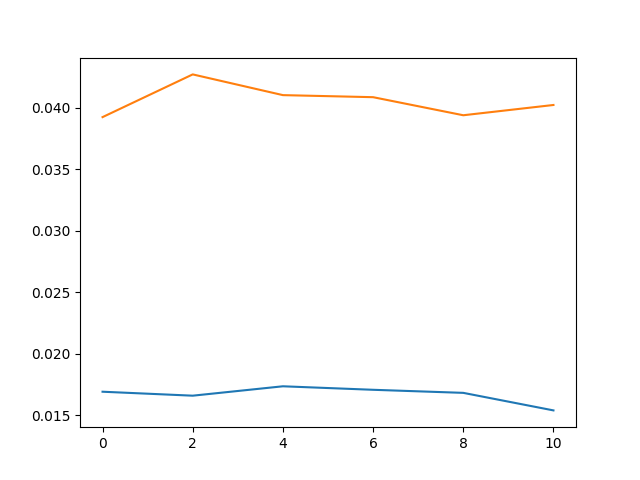
\includegraphics{tau_t.png}
        \caption{A realization of $\tau_1(t)$ (orange) and $\tau_2(t)$ (blue).}
        \label{fig:tau-realization}
    \end{figure}

    We would like to know how this Robust Model would perform in an actual realization.
    In order to answer this question,
    we will create a simulated realization of the task processing times.
    Define
    $\bar{\tau_j}(t) = \tau_j (1 + 0.5\zeta_j(t) \epsilon)$
    for $t \in [0,T]$,
    where $\zeta_j(t):[0,T] \to [0,1]$ is a stochastic process.
    In this experiment,
    we randomly generate $\zeta(t)$ by as a sum of four sinus functions of the form $h \sin(\pi f t + o)$,
    where $h$ is the amplitude,
    $f$ is a positive integer,
    increasing for each sine as $1,2,3,4$,
    and $o$ is a random phase shift taken  from $U(0,2\pi)$.
    We sum these up so that the total realized $\tau_j(t)$ are within the desired bounds as shown in \Cref{fig:tau-realization}.

    We generate realizations of $\zeta_j(t)$ once,
    and use them for all of the following steps
    to compute simulated realizations of $\bar{\tau_j}(t)$,
    which we call $\tau_j(t)$.
    We then compute the simulated buffer quantities using $\tau_j(t)$:

    \begin{align}
        \label{eq:buffer-robust-realization}
        \begin{split}
            x_1^R (t) &= 100 + 40 t \int_0^t \frac{\eta_1(s)}{\tau_1(s)} \dd s \\
            x_2^R (t) &= 100 + 20 t \int_0^t \frac{\eta_2(s)}{\tau_2(s)} \dd s
        \end{split}
    \end{align}

    The value of our objective is then:
    \begin{equation}
        \label{eq:cost-robust-realization}
        \int_0^T \left( x_1^R(t) + x_2^R(t) \right) \dd t
    \end{equation}
    which in our realization is $2614.53$.

    What if,
    instead of solving \modeltwo~ which is Bertsimas' sequencing-policy model,
    we solve our server-effort model,
    \modelone?

    Define,
    for classes $j=1,2$,
    $\mu_j=1/(\tau_j ( 1 - 0.5 \epsilon))$.
    This assumes we process jobs as fast as possible.
    But we must make sure we do not cause the queues to become empty.
    Adjust \modelone~ as follows:
    \begin{align}
        \label{eq:model-1-robust}
        \begin{split}
            \min\limits_{\eta_1, \eta_2}
            &~ \int_0^T \left( x_1(t) + x_2(t) \right) \dd t \\
            \text{s.t.}
            &~ 0 \leq \eta_1(t) + \eta_2(t) \leq 1 \\
            &~ x_1(t) = 100 - \int_0^t 63.16 \eta_1(s) \dd s + 40t \geq 0 \\
            &~ x_2(t) = 100 - \int_0^t 26.32 \eta_2(s) \dd s + 25t \geq 0
        \end{split}
    \end{align}

    Using the same realization as above,
    we e obtain the solution of $100\%$
    server effort on class 1 for $3.75$ hours,
    then $60\%$ on class 1 and $40\%$
    on class 2 for the remaining $6.25$ hours.
    We compute the buffer values using \Cref{eq:buffer-robust-realization} once again,
    and the objective using \Cref{eq:cost-robust-realization},
    this time obtaining a value of $2573.25$ for the same realization.
    This is an improvement over the objective value we obtained with \modelone.

    \begin{claim}
        \label{claim:modelone-better}
        For any realization $\tau^*(t)$ of $\bar{\tau}(t)$,
        define $Z_1$ as the objective from Robust \modelone,
        and $Z_2$ as the objective from Robust \modeltwo.
        Then $Z_1(\tau^*(t)) < Z_2(\tau^*(t))$.
    \end{claim}

    We plan to prove \Cref{claim:modelone-better} by comparing the feasible regions of the corresponding robust counterparts,and showing that the proposed model’s region contains the feasible region ofBertsimas’ model.

    We now suggest an alternative method of obtaining an optimal solution.
    Recall that the constraints in \Cref{ex:one-computer-two-classes-concrete}
    are of two kinds:
    server effort constraints,
    and buffer constraints.
    Our suggested method will solve the nominal case,
    which is the same as what we previously called the deterministic case,
    to obtain some rules for the optimal control of the server.
    However,
    we will apply some post-processing logic to the realization,
    where we allow the buffer value \textit{of the realization}
    to go below $0$.
    When it does,
    the server will apply $0$-effort to the corresponding job class.

    When we compute the objective function,
    we won't want to use any negative values in the buffers.
    In the mathematical model,
    the buffer values are allowed be negative,
    but when we translate them back to the physical system,
    we treat negative values as if they are zero.
    For this,
    we introduce the variables $\xi$ to represent this artificial buffer.
    Allowing the buffers to be negative increases the space of feasible solutions and therefore enables the possibility of an improved solution being found.

    \begin{align}
        \begin{split}
            \xi_1(t) & = 100 - \int_0^s 60 \eta_1(s) \dd s  + 40t \\
            \xi_2(t) & = 100 - \int_0^s 25 \eta_2(s) \dd s  + 20t
        \end{split}
    \end{align}

    Then we define, for $j=1,2$
    \begin{equation}
        x_j^R(t) =
        \begin{cases}
            \xi_j(t) & \xi_j(t) > 0 \\
            0 & \text{otherwise}
        \end{cases}
    \end{equation}.

    These variables cannot be negative,
    and so we can use them to compute the objective function.
    Using the same realization as above,
    we obtain the objective $2181.73$,
    which is not far off the deterministic value.

    \begin{claim}
        \label{claim:newmodel-converge}
        Define $Z^*$ as the objective obtained in our new proposed method,
        and $Z$ as the objective of the deterministic model.
        Then,
        for certain stochastic processes $\zeta(t)$,
        we have $\mathbb{E}(Z^*) \to Z$.
    \end{claim}

    We plan to prove \Cref{claim:newmodel-converge} by  finding how the distribution of the parameters propagates to the realized value of the objective function and to the realized solution. Alternatively, we can use a stochastic programming approach to show that the objective of the relaxed problem is better than that of the original problem.

    \clearpage
    \printbibliography
    \label{sec:bibliography}

\end{document}
